\addcontentsline{toc}{chapter}{Messdaten}
\label{Protokoll}

% \thispagestyle{empty}

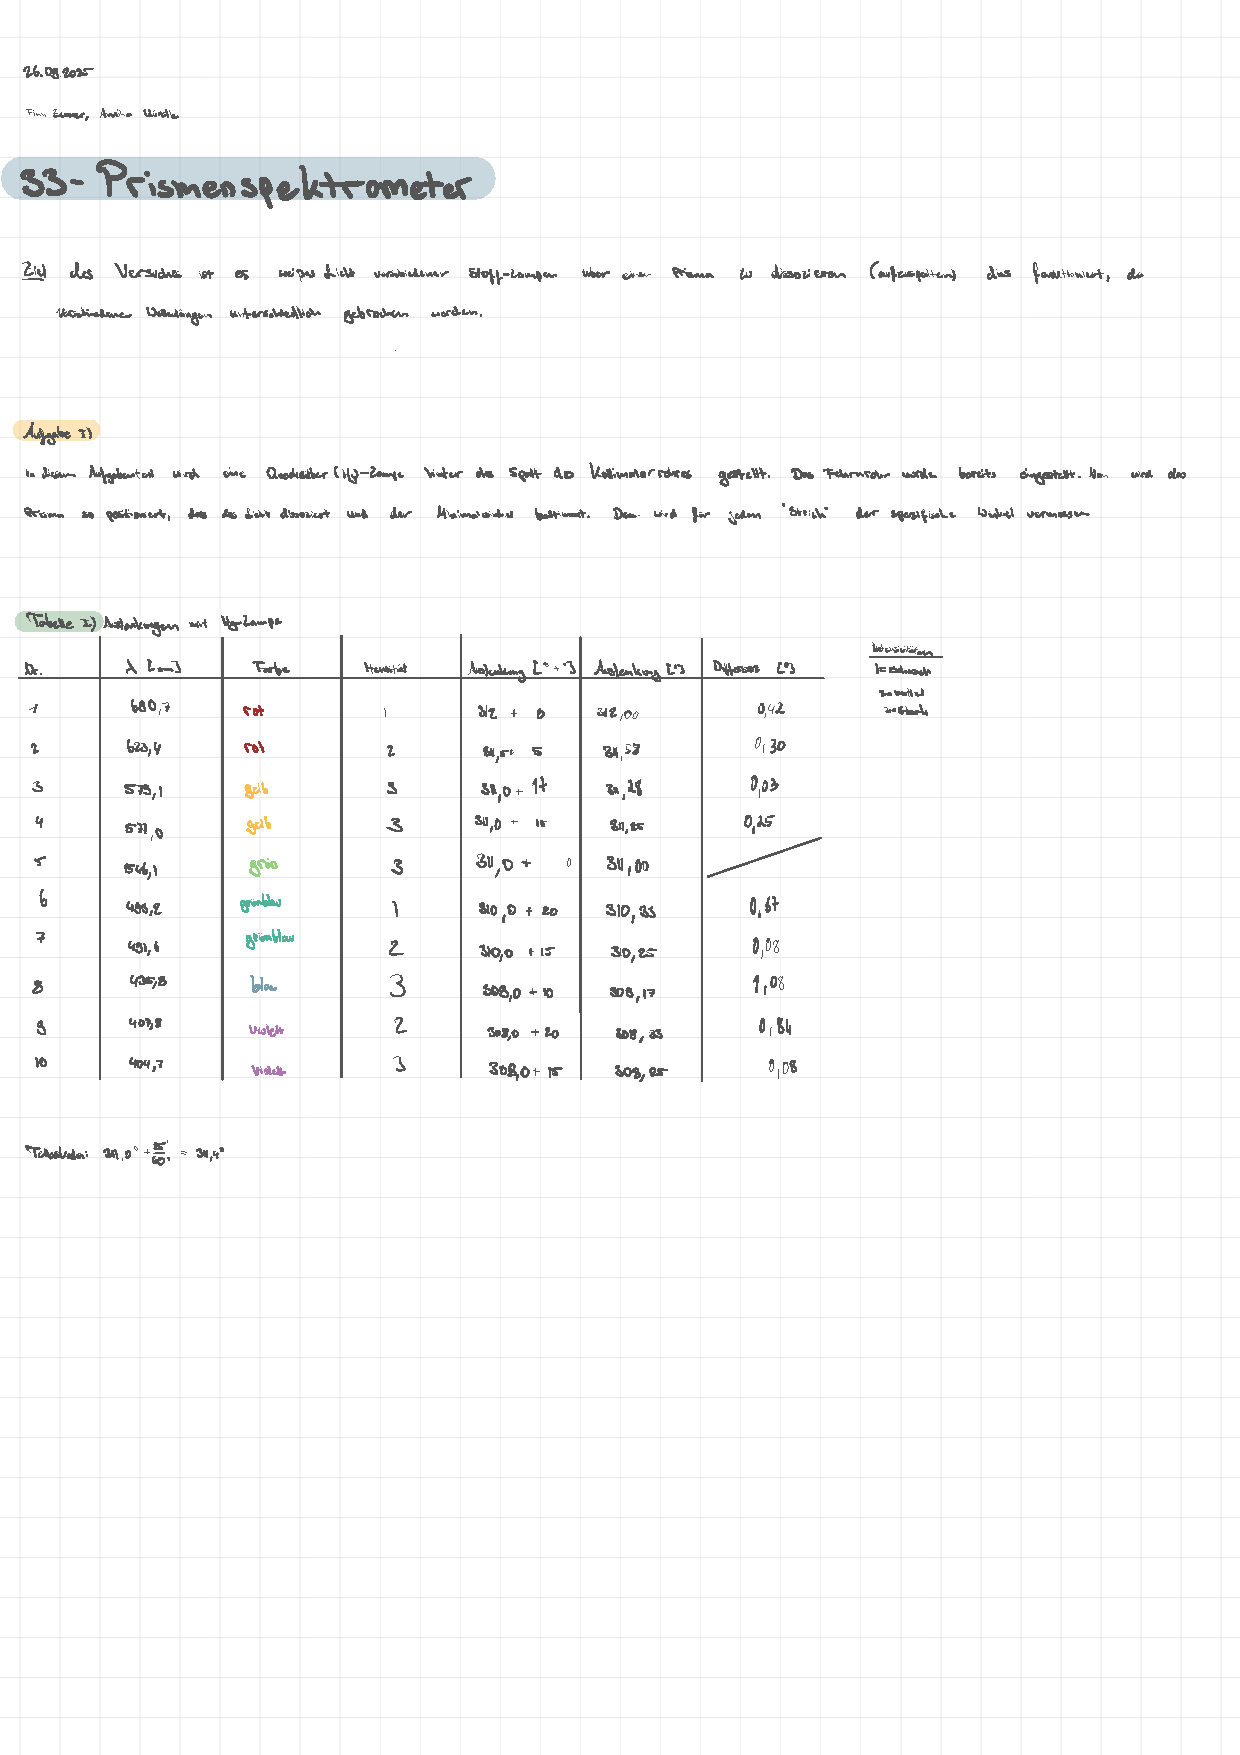
\includepdf[
  pages=-,               
  pagecommand={\thispagestyle{empty}} 
]{Protokolle/\versuchsnummer/Chapter/Messprotokoll.pdf}

\addcontentsline{lot}{table}{\protect\numberline{\thechapter.1} Scheibendrehung}
\addcontentsline{lot}{table}{\protect\numberline{\thechapter.2} Trägheitsmoment der regelmäßigen Messingplatte}
\addcontentsline{lot}{table}{\protect\numberline{\thechapter.3} Trägheitsmoment der unregelmäßigen Messingplatte}
\addcontentsline{lot}{table}{\protect\numberline{\thechapter.4} Schtein'scher Satz}
